
\chapter{Introduction}
\label{chap:introduction}

% two problems
In this thesis I address two current problems in the physics of solar wind: the prediction of the solar wind's geomagnetic impact, which is one of the most important key objectives in space weather, and the characterization of the solar wind conditions in the near-Sun region, which will be explored by the Parker~Solar~Probe mission beginning in end of 2018. These two problems are linked in view of the fact that the solar wind impacting the magnetosphere originates from the near-Sun region.

% two topics and studies
This thesis presents quantitative studies examining both topics. Despite a considerable difference with regard to their content, the two studies both share their predictive nature related to solar wind, deal with similar data sets, and harness similar data processing methods.
% response to problems
In the following, I introduce both topics separately. First, I lead into the subject of quantifying the solar wind's geomagnetic impact for different forecast situations. Second, I present the issue of estimating the near-Sun solar wind environment which Parker Solar Probe will encounter during its mission.

\bigskip

% chapter2: Kp estimate from sw

% 1) contextualizing background information
The Sun emits a continuous flow of magnetized plasma into space, which mainly consists of electrons and protons, and is called solar wind. This solar wind fills the interplanetary space and interacts with solar system bodies and their possible magnetospheres. It has been known since the early 19th~century that variations in the solar wind evoke disturbances in the terrestrial magnetosphere \citep{Bartels1962}.
% CMEs
Particularly strong disturbances, called geomagnetic storms, can be provoked by coronal mass ejections (CMEs), which consist of magnetically structured coronal plasma shot into the ambient solar wind by rearrangements in the configuration of the solar magnetic field. One of the latest CMEs generating strong geomagnetic storms is displayed in the coronagraph image in \autoref{fig:SOHO_LASCO_C3_20170906_151807}. The impact of CMEs on the Earth's magnetosphere can be significantly stronger than that of the ambient solar wind streams, owing to the potentially extreme values of their properties, such as magnetic field strength and velocity, which are able to be several times higher than those of ambient streams.
\begin{figure}[htb]
	\fcapside[\FBwidth]{
		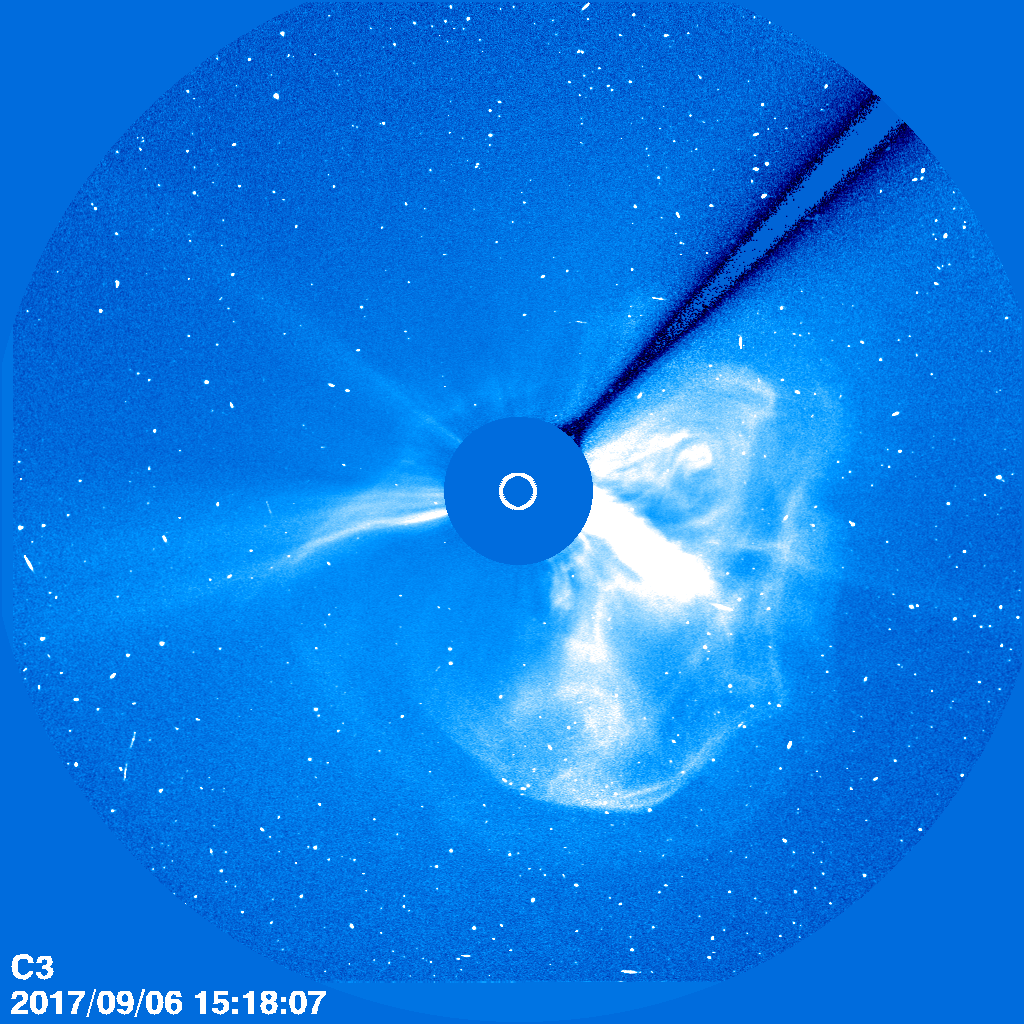
\includegraphics[width=0.5\textwidth]{figures_of_others/images/SOHO_LASCO_C3_20170906_151807.png}
	}{
		\caption[\lofimage{figures_of_others/images/SOHO_LASCO_C3_20170906_151807.jpg}Courtesy of SOHO/LASCO consortium; SOHO is a project of international cooperation between ESA and NASA.]
		{White-light image of the solar corona out to \SI{30}{\Rs} from 6~September 2017 taken by the LASCO/C3 coronagraph on board the SOHO spacecraft. The solar disk's position is indicated by the white circle. Thedisk is covered by an occulter disk with a mount to the top right. The bright extensive structure is the CME and the faint aura around is a shock wave. Courtesy of SOHO/LASCO consortium; SOHO is a project of international cooperation between ESA and NASA.}
		\label{fig:SOHO_LASCO_C3_20170906_151807}
	}
\end{figure}
% LASCO movie tool
% https://lasco-www.nrl.navy.mil/index.php

% consequences
The effects of geomagnetic storms pose a threat both to exposed humans and sensitive technological systems. The potential disruption of critical systems, such as satellite communication and power grids, would not only have severe economic implications but would affect human lives as well. The rapid rate of technological advancement leads to an ever-growing abundance of systems which are sensitive to disturbances in the geomagnetic field. Therefore, it is becoming increasingly important to be capable of predicting the onset of magnetospheric disturbances and their magnitude, in order to mitigate such severe consequences.

\pagebreak

% what is well known
As a result of solar wind in-situ measurements, it is well known that variations in specific solar wind quantities lead to direct responses in geomagnetic activity. The coupling mechanisms between solar wind and magnetosphere have been identified and modeled extensively, resulting in a variety of coupling functions linking solar wind parameters to indicators of geomagnetic activity. These coupling functions serve as the basis for models that predict geomagnetic activity from solar wind input parameters and thus, knowledge of the solar wind conditions in front of the magnetosphere enables to predict the geomagnetic response fairly well.

% 2) problem statement
The solar wind is continuously monitored in~situ by spacecraft located in front of the magnetosphere. These real-time measurements are used by operational space weather services for providing nowcasts of geomagnetic activity. The monitoring spacecraft are located at the first Lagrange point (L1), which is situated at approximately one-hundredth the distance from the Earth to the Sun.
Solar wind plasma from this point reaches the magnetosphere in a few tens of minutes, which is significantly shorter than its  travel time from Sun to Earth, which is around three to four days for ambient solar wind streams and about a day for extremely fast CMEs.
In order to exploit this extended lead time, some information about CMEs and solar wind streams can be acquired from remote observations provided by solar imagers and coronagraphs. The velocity is one of the few remotely acquirable quantities which is to a certain degree reliably forecastable.
Space weather nowcast services reach a high prediction accuracy by using in-situ measurements from L1, however, for remote forecast situations the methods used by nowcast services are not effective, because not all solar wind parameters necessary for geomagnetic activity forecasts can readily be obtained.

% 3) response to the problem
This study addresses this problem in that it quantifies the geomagnetic response for remote forecast situations, when only the velocity information from CMEs or ambient solar wind is available.
The present study relates the planetary geomagnetic disturbance indicator \Kp{} with velocity measurements made ahead of the Earth's magnetosphere. In view of the differences between the velocity prediction methods applied for CMEs and streams, I derive separate relations for CME-associated flows and for solar wind streams. This study is based on 35~years of solar wind data from the hourly OMNI data set and on the classification from the list of Solar Wind Structures (SWS).
Solar wind analyses in conjunction with \Kp{} commonly employ averaged solar wind data, even though the \Kp~index represents the value of the maximal geomagnetic disturbance per 3"~hour interval and not its average -- the underlying time resolution is 1~minute. Thus, a unique approach in the present study is the use of 3"~hour extreme values derived from minutely solar wind data. This method is therefore expected to result in significantly enhanced correlations between the \Kp~index and solar wind data. Here, this approach is tested and compared for the cases of the solar wind electric field, which represents one of the most prominent coupling functions, and the velocity.

% purpose statement
The purpose of this study is to provide empirical \Kp{} relations that can be utilized in specific forecast situations when only the remotely estimated velocities of CMEs or streams are known.
The study further shows the impact of the way the high-resolution solar wind data is processed to 3"~hourly values by means of the \Kp{} relations to the electric field and the velocity.

\bigskip

% chapterPSP: sw estimate from Helios
In the following, I introduce the second topic of this thesis.
% 1) contextualizing background information
The solar wind was first theoretically described by \citet{Parker1958} who formulated a model of an expanding isothermal solar atmosphere. His model describes a continuous supersonic radial outflow of magnetized plasma and the consequences for the structure of the heliospheric magnetic field. The existence of this solar wind was subsequently confirmed from in-situ measurements made by the first satellites in 1959. Since then, solar wind measurements were made almost continuously by various spacecraft located near Earth. By now, the solar wind is measured throughout the heliosphere -- the two Voyager probes tracked it from Earth to the outer solar system, the Ulysses spacecraft charted the solar wind up to high heliolatitudes, and the two Helios spacecraft measured it from Earth down to the solar distance of Mercury.

% 2) problem statement
However, the region close to the Sun remains unexplored although it is of particular scientific interest. In this region, the corona is heated to temperatures far exceeding those of the underlying photosphere and the plasma is being accelerated to its final solar wind speeds. Up to now the mechanisms that heat the corona and accelerate the solar wind are still not fully understood.
As this region is assumed to hold the answers to these open key questions, it has long been planned to send a probe to this region. The Parker Solar Probe (PSP) mission is intended to address these questions. The PSP spacecraft, launched on 12~August 2018, will dive through the corona within distances down to \num{8.86}~solar radii (\Rs) from the solar surface, see \autoref{fig:SPP_ObservingSun2b}. It will provide for the first time in-situ measurements and high-resolution images of the solar wind conditions in this unexplored region.
\begin{figure}[htb]
	\fcapside[\FBwidth]{
		\includegraphics[width=0.6\textwidth]{figures_of_others/images/SPP_ObservingSun2b.jpg}
	}{
		\caption[\lofimage{figures_of_others/images/SPP_ObservingSun2b.jpg}Credit: \href{http://parkersolarprobe.jhuapl.edu/Multimedia/Images.php}{NASA/Johns Hopkins APL/Steve Gribben}, 2018.]
		{Artist’s rendering of the PSP spacecraft approaching the Sun. Close to the Sun, the heat shield will actually always point in direction of the Sun. Credit: \href{http://parkersolarprobe.jhuapl.edu/Multimedia/Images.php}{NASA/Johns Hopkins APL/Steve Gribben}, 2018.}
		\label{fig:SPP_ObservingSun2b}
	}
\end{figure}

% 3) response to the problem
This study addresses this topic in that it explores the near-Sun solar wind conditions and predicts the solar wind environment for the PSP orbit, that is, this work derives estimates of the key solar wind parameters magnetic field strength, proton velocity, density, and temperature. These key parameters are back-extrapolated to the near-Sun region, using an empirical solar wind model for the inner heliosphere.
\pagebreak
I develop this solar wind model from solar activity and solar distance dependencies of each parameter individually. To derive the dependencies on solar activity, solar wind measurements from the near-Earth OMNI data set are being related to the sunspot number. To derive the solar distance dependencies, I apply solar wind data from the Helios~1 and Helios~2 probes, which flew in the 1970s and took in-situ measurements between \SI{0.29}{\au} and \SI{0.98}{\au}.
Commonly, studies that analyze solar wind handle it by working with time averages of the bulk parameters. In contrast, the special approach in this work is its tackling of the frequency distributions. The model represents the solar wind parameters by lognormal distributions, furthermore, both the slow and fast velocity components are taken into account.
For the magnetic field strength, I additionally derive a second alternative distance dependency that is based on the Parker magnetic field geometry.

% purpose statement
The purpose of this study is to quantitatively model the key solar wind parameters in the inner heliosphere, to estimate the near-Sun solar wind environment, and further to predict it in particular for the orbit of the PSP spacecraft.
% what will be addressed\\
% what not; what lies outside the scope of this thesis\\

\bigskip

%Synopsis	% Outline (chapters and their content)
I structured this document as follows: \autoref{chap:basics} lays out the fundamentals behind the problems addressed in this work as well as the current state of research. This comprises basic knowledge about the Sun, its activity and magnetic field, solar wind, space weather, magnetosphere, geomagnetic activity and forecast methods. \autoref{chap:data} describes those instrumentation and data sources on which the studies in the subsequent chapters are based on. \autoref{chap:chapter2} presents the analyses performed on the solar wind's magnetospheric influence, with focus on predicting the \Kp~index from the solar wind electric field and from the velocities of CMEs and streams. \autoref{chap:chapterPSP} is followed by the published article on the same topic, integrated as \autoref{chap:solar_wind_predictions_for_the_parker_solar_probe_orbit} into this document. These chapters develop an empirical solar wind model for the inner heliosphere and use it to estimate the near-Sun solar wind environment of the PSP mission underway. The model comprises the solar wind parameters magnetic field strength, proton velocity, density, and temperature. Furthermore, an alternative magnetic field model is outlined, which exhibits a solar distance dependency based on Parker's magnetic field formulation. Eventually, \autoref{chap:summary} offers a summary of the results and conclusions, and gives an outlook on ideas for further studies. The subsequent \autoref{chap:appendix} contains helpful information and theory about several more specific topics, as well as a list of frequently used acronyms in this work in \autoref{sec:acronyms}.


